\documentclass[12pt,letterpaper]{article}
\usepackage{fullpage}
\usepackage[top=2cm, bottom=4.5cm, left=2.5cm, right=2.5cm]{geometry}
\usepackage{amsmath,amsthm,amsfonts,amssymb,amscd}
\usepackage{lastpage}
\usepackage{enumerate}
\usepackage{fancyhdr}
\usepackage{mathrsfs}
\usepackage{xcolor}
\usepackage{graphicx}
\usepackage{hyperref}
\usepackage{sectsty}
\usepackage{enumitem}
\usepackage{siunitx}
\usepackage{subfig}
\usepackage{stackengine}


\sectionfont{\fontsize{14.4}{17}\selectfont}
\subsectionfont{\fontsize{10}{12}\selectfont}

\hypersetup{%
  colorlinks=true,
  linkcolor=blue,
  linkbordercolor={0 0 1}
}

\setlength{\parindent}{0.0in}
\setlength{\parskip}{0.05in}

% Edit these as appropriate
\newcommand\course{CMPE 670}
\newcommand\hwnumber{1}
\newcommand\NetIDa{Andrei Tumbar}

\pagestyle{fancyplain}
\headheight 35pt
\lhead{\NetIDa}
\chead{\textbf{\Large Homework \hwnumber}}
\rhead{\course \\ \today}
\lfoot{}
\cfoot{}
\rfoot{\small\thepage}
\headsep 1.5em

\begin{document}

\section*{Question 1}

\begin{enumerate}[label=\alph*)]
  \item
   Layer is the idea in which a system is divided into smaller and simpler
   portions which in turn simplified a problem into a simpler set of problems.
   Each layer will perform some sort of processing to the original
   data and pass it on to lower layers. After the data has been processed by the
   lowest layer, it is passed to the receiving device where the data is unpacked
   from the lowest to highest layers in order. Using layered architecture will also
   allow changes to the design or operation of a single layer without impacting
   other layers.
  \item
   The network protocol was designed in seven layers for a variety of reasons.
   Firstly, while more layers would allow for lower complexity in each layer,
   layers needs to interface with their direct siblings above and below.
   The creation of these interfaces is not trivial and therefore the number of
   layers should be kept to a reasonable count. Secondly, when choosing the functionality
   of each layer, similar functional steps in the communication process are
   grouped up abstract the process. Thirdly, by abstracting each step into layers,
   changes can be made to the operation of a single layer while not affecting other ones.
   Fourthly, engineers took into account previous networking experience to decide where
   the boundaries between different layer would go. Finally, engineers created layers
   where they expected interfaces to be standardized in the future.
\end{enumerate}

\section*{Question 2}
\subsection*{RRC (Radio Resource Control)}
The radio resource control later of the LTE architecture is the most difficult
layer to classify in terms of the OSI model. It has a wide range of functionality
mostly pertaining to that of the session layer. The key management for encryption
as well as mobility and QoS functionality are not explicitly defined by the OSI
model, however, they are related to session management.

\subsection*{PDCP (Packet Data Convergence Protocol)}
The PDCP layer will provide a protocol to send and receiving acknowledgment
units as well as provide data integrity checks on these units. It is mostly draws
from aspects described in the data link layer of the OSI model.

\subsection*{RLC (Radio Link Control)}
The RLC layer will segment the data into packets and verify in-sequence delivery
of these packets. The OSI model would group together some of the functionality of
the PDCP and RLC layers to formulate the data link layer.

\subsection*{MAC (Medium Access Control)}
Manages the physical connection by scheduling the sending and receiving of
packets. Incorporates parts of the data link and physical layers in the OSI model.

\subsection*{Wireless mobile connections}
Wireless mobile connections are especially vulnerable to cyber attacks because their
data is being transmitted through a public medium at long range. This means a potential
attacker may "listen in" on messages transmitted through mobile protocols. Security and
encryption has a much stronger emphasis in the mobile network architecture that previously
noted in the OSI model. While data integrity is something that both the wired and mobile
links need to take into account, ciphering to verify packet integrity is not explicitly
defined in the OSI model. The LTE PDCP layer will request re-transmission of a packet if
it cannot be verified against its cipher.

\section*{Question 3}
\subsection*{Part 1}
In the worst case scenario of the described problem, the packet would need to wait
for the transmission delay of two other $\SI{10}{kb}$ at each of the three
routers.

There are four physical lines connecting the sender and receivers via the three
intermediate routers. The total transmission time can then be calculated between
the start of the message being sent until the message has been fully received by
the receiver.

We start with the basic equations and definitions of nodal delay:
\begin{align}
d_{nodal} &= d_{proc} + d_{queue} + d_{trans} + d_{prop} \\
d_{proc} &\approx 0 \\
d_{queue} &= d_{trans} * n_{packets\_in\_queue} \\
d_{trans} &= L_{packet\_length} / R_{link\_bandwidth} \\
d_{prop} &= d_{line\_length} / s_{prop\_speed} 
\end{align}

Equation 2 shows a negligible time delay for the processing of each packet. This
is due to the sub-millisecond delay seen during this step.
Equation 3 was derived with this question in mind. The message in question needs
to wait for the transmission delay of two other 10k messages at each of the three
intermediate routers.

We can therefore arrive at an expression for the entire packet transmission:
\begin{align*}
d_{total} &= d_{trans\_sender} + d_{physical\_line} + 3d_{router} \\
&= d_{trans} + \SI{1000}{km}/\SI{0.3}{\km\per\us} + 3d_{queue} + 3d_{trans} \\
d_{trans} &= \SI{80000}{bits} / \SI{10}{Mpbs} = \SI{8}{\ms} \\
d_{queue} &= \SI{8}{\ms} * \SI{2}{packets} = \SI{16}{\ms} \\
d_{total} &= \SI{8}{\ms} + \SI{3.33}{\ms} + 3\cdot\SI{16}{\ms} + 3\cdot\SI{8}{\ms} = \pmb{\SI{83.33}{\ms}}
\end{align*}

\subsection*{Part 2}
The receiver needs to a send a message early enough so that during the time
taken for the message to reach the transmitter, the receiver cannot receive
more data that it can handle. This concept is called the bandwidth-delay product.

\begin{align*}
d_{delay\_total} \cdot R_{link\_bandwidth} &= n_{buffer\_bits} \\
\SI{83.33}{ms} \cdot \SI{10}{Mpbs} &= n_{buffer\_bits} \\
\SI{83.33e-3}{s} \cdot 2 \cdot \SI{10e6}{bps} &= \SI{1.667}{Mbit} = \pmb{\SI{208.375}{kbytes}}
\end{align*}

Another way to describe this byte count is the maximum number of bytes that
can be received during the time it takes a message to travel from the receiver
to the transmitter. The result is multiplied by $2$ because we must take into account
the delay for a round-trip instead of a single direction.

\section*{Question 4}

To calculate the minimum link capacity we start with the transmission delay
at each intermediate node as well as their definitions based on the question:
\begin{align*}
d_{nodal} &= d_{proc} + d_{queue} + d_{trans} + d_{prop} \\
d_{proc} &= 0 \\
d_{trans} &= L_{packet\_length} / R_{link\_bandwidth} = \frac{\SI{1}{Mbytes}}{R}(\frac{\SI{8}{bits}}{\SI{1}{byte}}) = \frac{\SI{8}{Mbits}}{R} \\
d_{queue} &= d_{trans} * n_{packets\_in\_queue} = d_{trans} * 4 \\
d_{prop} &= d_{line\_length} / s_{prop\_speed} = \frac{\SI{200e3}{m}}{\SI{2e8}{\m/\s}} = \SI{1}{ms}
\end{align*}

With the expression for the delay at each node described in terms of the link bandwidth,
$R$, an expression is derived in terms of a single node $d_{nodal}$.

\begin{align*}
\SI{1}{s} = d_{total} &= d_{trans} + d_{prop} + 2 \cdot d_{nodal} \\
&= \frac{\SI{8}{Mbits}}{R} + \SI{1}{ms} + 2(0 + 4\frac{\SI{8}{Mbits}}{R} + \frac{\SI{8}{Mbits}}{R} + \SI{1}{ms}) \\
\SI{1}{s} &= 11\frac{\SI{8}{Mbits}}{\SI[parse-numbers = false]{R}{Mbps}} + \SI{0.003}{s} \\
R &= \pmb{\SI{88.265}{Mbps}} 
\end{align*}

\section*{Question 5}
\subsection*{Part a}

\begin{figure}[h!]
\centering
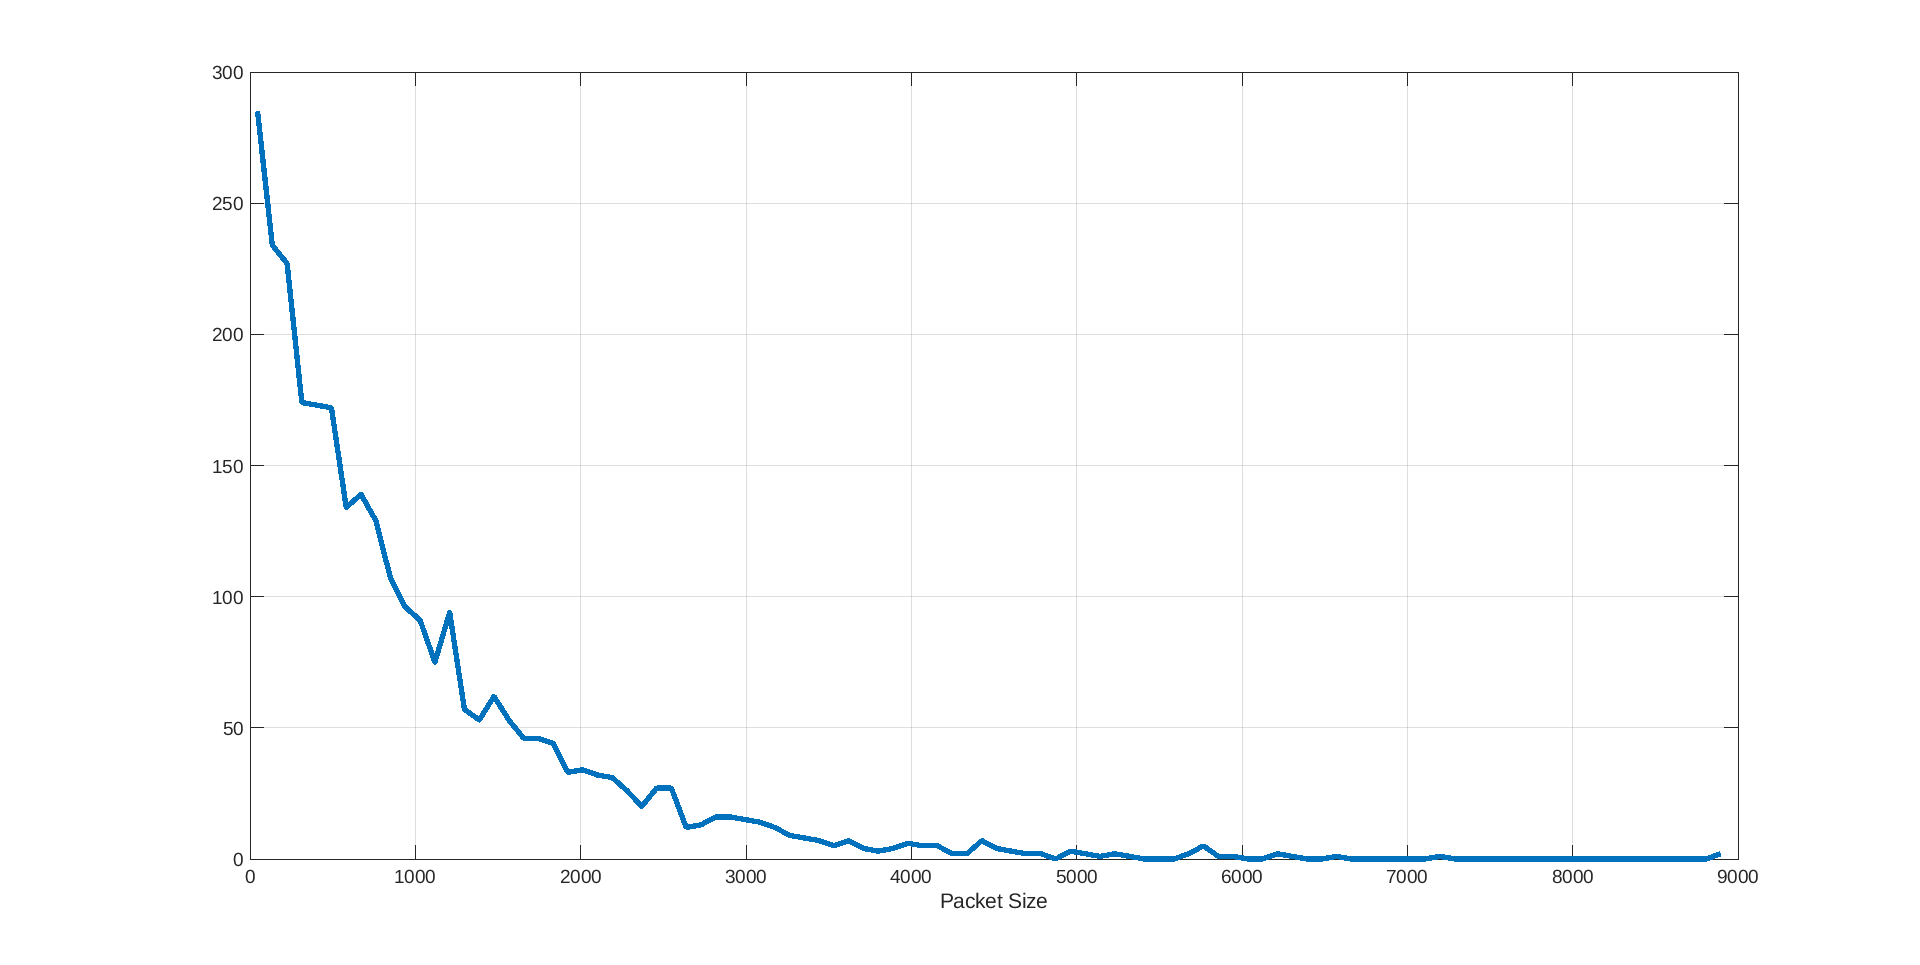
\includegraphics[width=5.5in]{figure1.png}
\caption{Plot showing the packet size distribution passing through Node 4.}
\label{fig:pa}
\end{figure}

Figure \ref{fig:pa} shows an exponential distribution of the of the packet
sizes passing through Node 4 of the simulated network.

\subsection*{Part b}

Using the matlab simulator, a variety of bitrates were tested on Node 4 to analyze the
effect that service rate has on the internal packet queue of a routing node.

\pagebreak

\begin{table}[h!]
    \renewcommand{\arraystretch}{1.3}
    \setlength{\tabcolsep}{12pt}
    \begin{center}
        \begin{tabular}{|c|c|c|}\hline
        Bitrate & Time spent in Node 4 & Average queue length (packets)\\\hline
        \SI{450}{kbps} & \SI{0.2588}{s} & 167.6696 \\\hline
        \SI{555.556}{kbps} & \SI{0.0128}{s} & 9.8181 \\\hline
        \SI{600}{kbps} & \SI{0.0107}{s} & 5.3916 \\\hline
        \SI{666.667}{kbps} & \SI{0.0060}{s} & 2.9483 \\\hline
        \SI{750}{kbps} & \SI{0.0040}{s} & 2.0296 \\\hline
        \SI{1}{Mbps} & \SI{0.0022}{s} & 1.0651 \\\hline
        \SI{1.5}{Mbps} & \SI{0.0011}{s} & 0.5692 \\\hline
        \SI{2}{Mbps} & \SI{0.00071}{s} & 0.3539 \\\hline
        \end{tabular}
    \end{center}
    \label{tab:tim}
\end{table}

The queue length inside Node 4 is graphed as a function of time for all of the
service bitrates in question.

\begin{figure}[h!]
  \begin{tabular}{cc}
    \stackunder{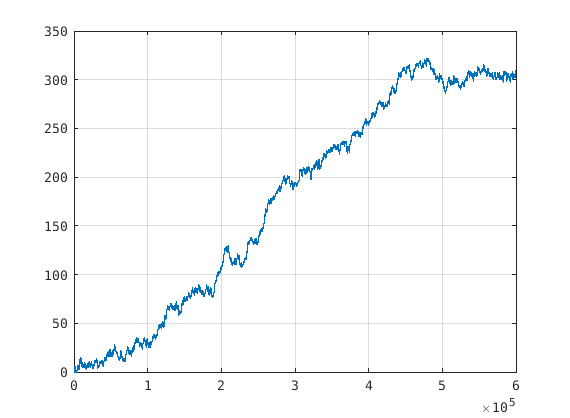
\includegraphics[width = 3in]{q_450k}}{\SI{450}{kbps}} &
    \stackunder{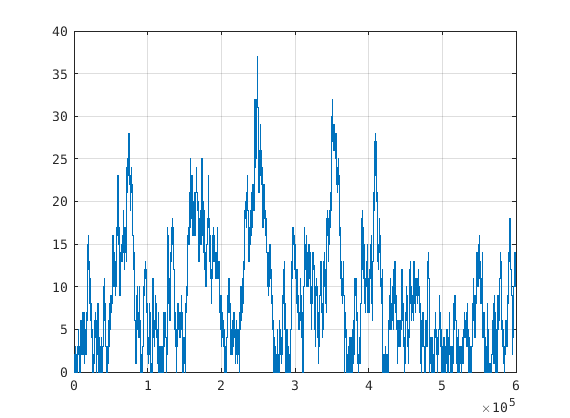
\includegraphics[width = 3in]{q_555_556k}}{\SI{555.556}{kbps}}\\
    \stackunder{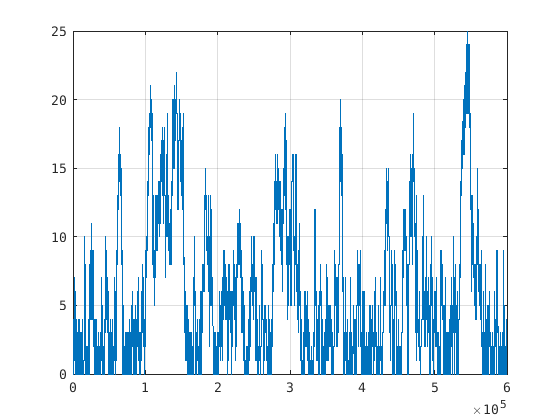
\includegraphics[width = 3in]{q_600k}}{\SI{600}{kbps}} &
    \stackunder{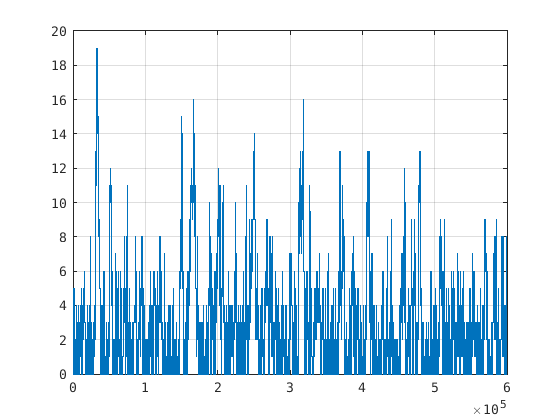
\includegraphics[width = 3in]{q_666_667k}}{\SI{666.667}{kbps}}\\
  \end{tabular}
\end{figure}

\pagebreak

\begin{figure}[h!]
  \begin{tabular}{cc}
    \stackunder{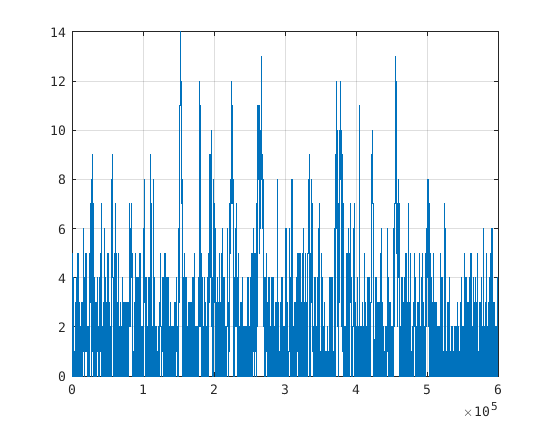
\includegraphics[width = 3in]{q_750k}}{\SI{750}{kbps}} &
    \stackunder{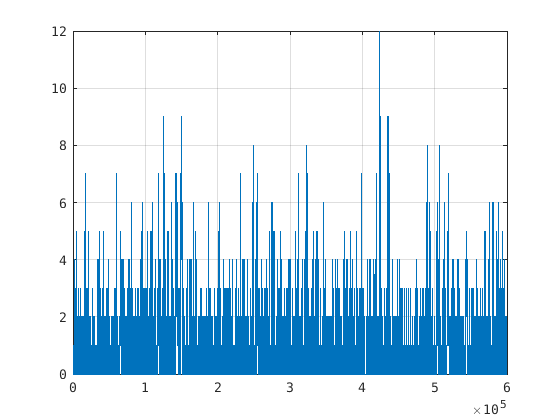
\includegraphics[width = 3in]{q_1m}}{\SI{1}{mbps}}\\
    \stackunder{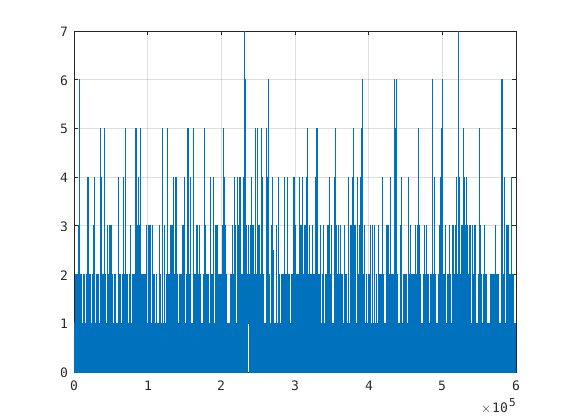
\includegraphics[width = 3in]{q_1_5m}}{\SI{1.5}{mbps}} &
    \stackunder{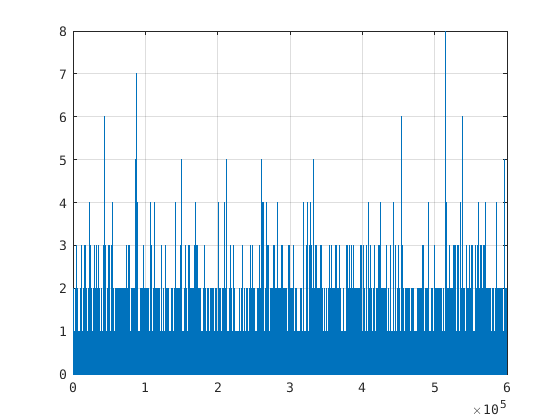
\includegraphics[width = 3in]{q_2m}}{\SI{2}{mbps}}\\
  \end{tabular}
\end{figure}

In reality, the queue size of a node inside a network is bounded by the maximum size
of the queue. Any overflow will result in dropped packets. For the sake of the this
example however, the number of packets inside a queue will not increase to infinity
if the service rate is faster than arrival rate. This is because packets are processed
and sent out faster than they can be received. According to the plots above, the only
service rate that increase without bound is the \SI{450}{kbps} service rate. Looking at
the higher service rates, while packets do not accumulate inside the queue, higher service
will accumulate fewer packets on average because the node is able to transmit each packet
faster.

\pagebreak

\subsection*{Part c}

Using the data from Part B, the mean time spend in Node 4 was plotted as a function
of service rate. The \SI{450}{kbps} point was omitted because it operated under a
different set of rules.

\begin{figure}[h!]
  \centering
  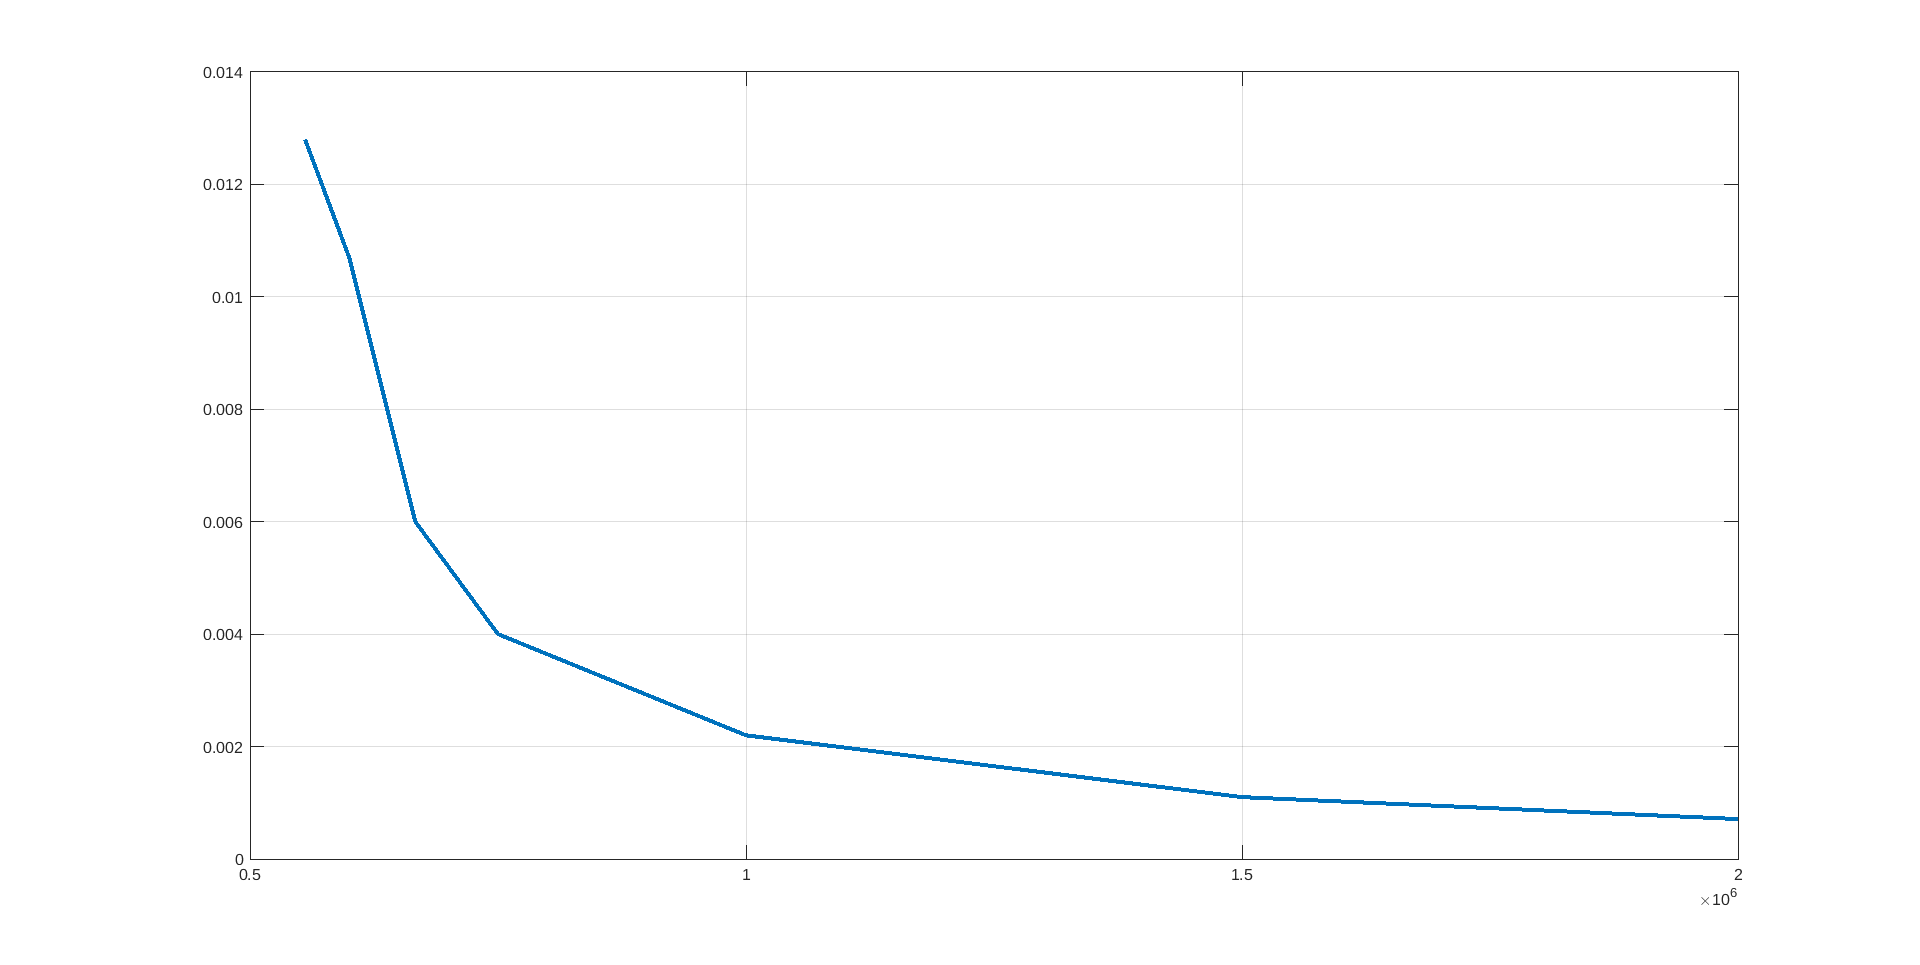
\includegraphics[width = 5in]{mean_time}
  \caption{Time in node (seconds) vs service rate (mbps)}
  \label{fig:pc}
\end{figure}

According to Figure \ref{fig:pc}, as the service rate decreases approaching 
500 kbps, the time in the node approaches infinity because the node cannot
process the data fast enough to keep up with the incoming data.

\pagebreak

\subsection*{Part d}

Using the data from Part B, the average queue length in Node 4 was plotted as a function
of service rate. The \SI{450}{kbps} point was omitted because it operated under a
different set of rules.

\begin{figure}[h!]
  \centering
  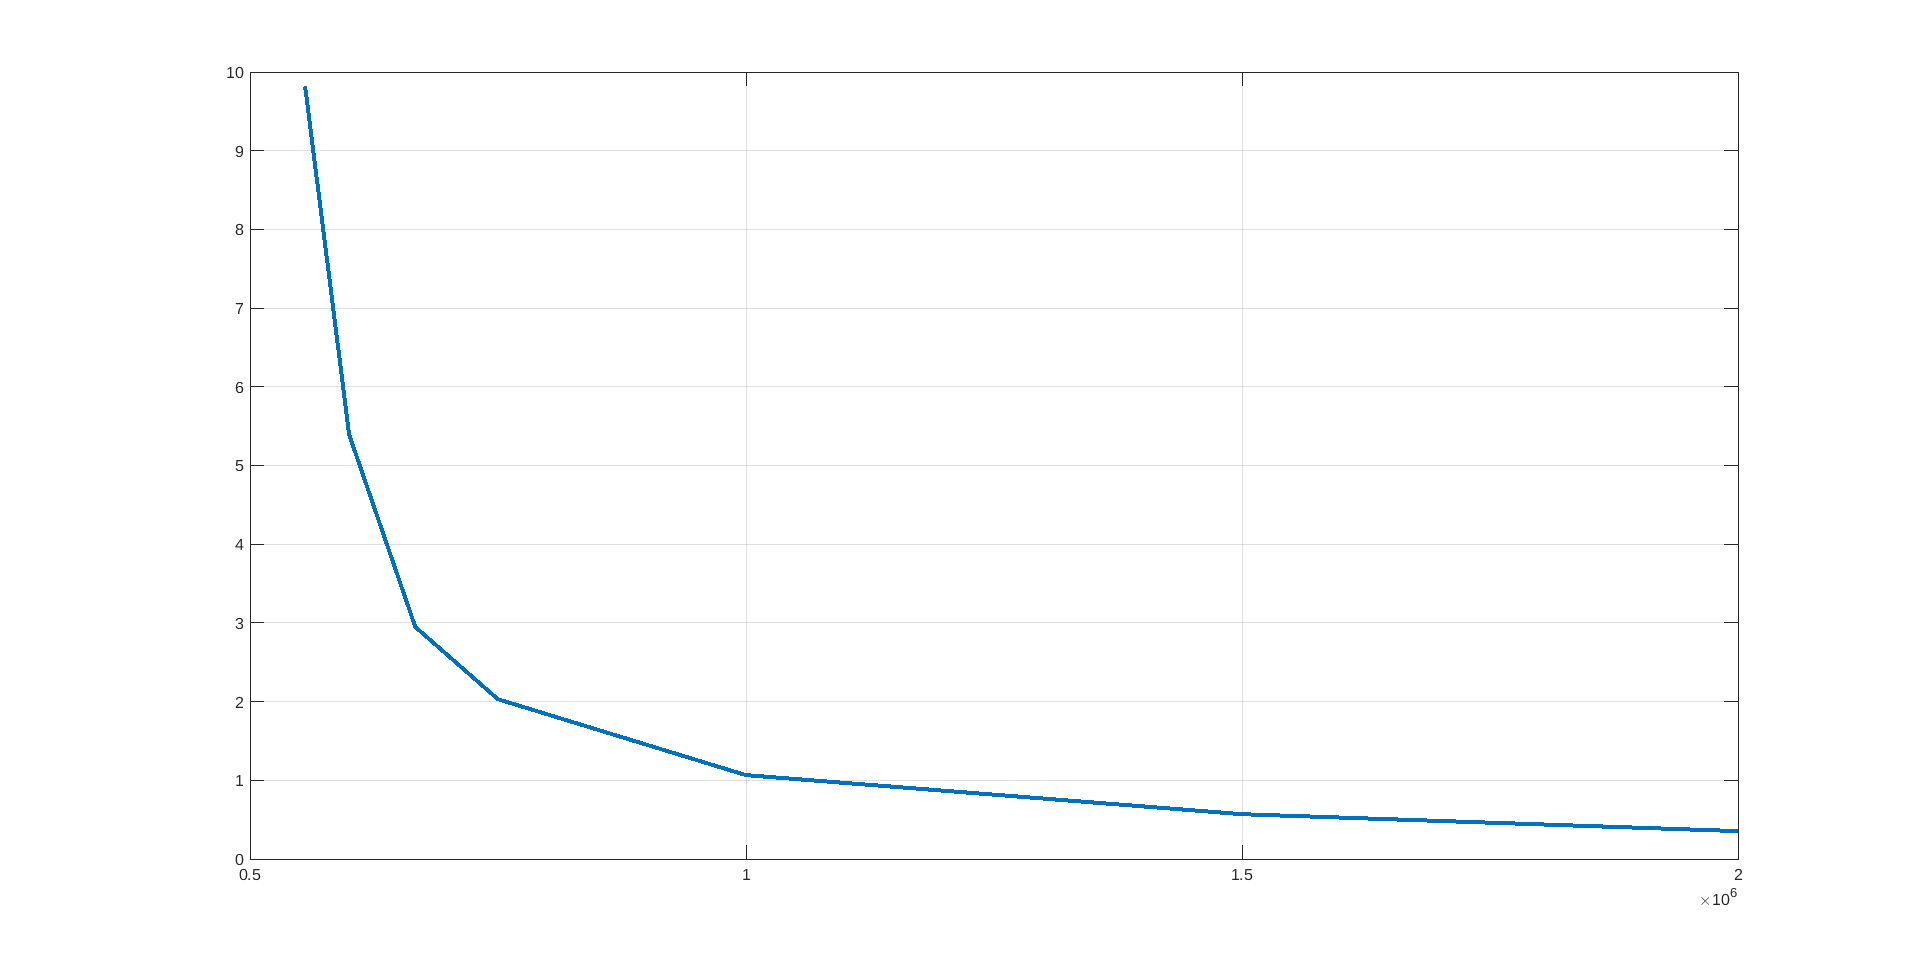
\includegraphics[width = 5in]{mean_length}
  \caption{Queue length (packets) vs service rate (mbps)}
  \label{fig:ql}
\end{figure}

The results shown in Figure \ref{fig:ql}, the queue length will behave similarly to
the time spend in the node. As the service rate approaches \SI{500}{kbps}, the queue
length will approach infinity.

\end{document}
